\documentclass{article}

\usepackage{graphicx}
\usepackage{fancyhdr}
\usepackage[margin=1in]{geometry}
\usepackage{listings}
\usepackage[hidelinks]{hyperref}
\usepackage{subfigure}
\usepackage{amsmath}
\usepackage{subcaption}
\usepackage{float}

\hypersetup{
	colorlinks=true,
	linkcolor=teal,
	filecolor=magenta,      
	urlcolor=teal,
	citecolor = teal
}
\usepackage{xcolor}
\usepackage{xepersian}
\setlength\headheight{28pt} 
\settextfont[
    Path = ./font/, % specify the path to the font files
    Scale = 1.3,
    UprightFont = XB Niloofar, % Regular font
    BoldFont = XB NiloofarBd,       % Bold font
    ItalicFont = XB NiloofarIt,   % Italic font
    BoldItalicFont = XB NiloofarBdIt % Bold Italic font if available
]{XB Niloofar}
\setlatintextfont[Scale=1]{Times New Roman}
\renewcommand{\baselinestretch}{1.5}
\pagestyle{fancy}
\fancyhf{}
\rhead{
\includegraphics[width=1cm]{img/Logo.png} 
	یادگیری ماشین
	-
	مینی پروژه شماره 2}
\lhead{\thepage}
\rfoot{سیدمحمد حسینی}
\lfoot{9821253}
\renewcommand{\headrulewidth}{1pt}
\renewcommand{\footrulewidth}{1pt}
\renewcommand{\lstlistingname}{Code}

\definecolor{codegreen}{rgb}{0,0.6,0}
\definecolor{codegray}{rgb}{0.5,0.5,0.5}
\definecolor{codepurple}{rgb}{0.58,0,0.82}
\definecolor{backcolour}{rgb}{0.95,0.95,0.92}

\lstdefinestyle{mystyle}{
	backgroundcolor=\color{backcolour},   
	commentstyle=\color{codegreen},
	keywordstyle=\color{magenta},
	numberstyle=\tiny\color{codegray},
	stringstyle=\color{codepurple},
	basicstyle=\ttfamily\footnotesize,
	breakatwhitespace=false,         
	breaklines=true,                 
	captionpos=b,                    
	keepspaces=true,                 
	numbers=left,                    
	numbersep=5pt,                  
	showspaces=false,                
	showstringspaces=false,
	showtabs=false,                  
	tabsize=2
}

\lstset{style=mystyle}

\begin{document}
	
	\begin{titlepage}
\begin{center}
\defpersianfont\nast[Path={./font/}, Scale=2]{IranNastaliq}
\centerline{{
\includegraphics[width=5cm]{img/Logo.png}}}
\centerline{\textcolor[rgb]{0,0,0.5}{\nast \large  دانشگاه صنعتی خواجه نصیرالدین طوسی}}
\centerline{\textcolor[rgb]{0,0,0.5}{\nast \bfseries دانشکدۀ مهندسی برق - گروه مهندسی کنترل}}

\vfill
        
\Huge
\textbf{یادگیری ماشین}\\
\textbf{پاسخ مینی پروژه دوم}\\
        
\vfill
\large
    نام و نام خانوادگی:  سیدمحمد حسینی\\
    شمارۀ دانشجویی: 9901399\\
    تاریخ: مهرماه 1402\\

\href{https://github.com/mamdaliof/MachineLearning2024W}{GitHub}

\href{https://drive.google.com/drive/folders/10-8uiqpIUbC2HcEtwjqP1IAix46nCrbL?usp=sharing}{Google Drive}


\end{center}
\end{titlepage}

	
	\tableofcontents \clearpage
	\listoffigures \clearpage
	\listoftables \clearpage
	\lstlistoflistings \clearpage
	\newpage
	
	\section{ سوال اول}\label{Section1}
	\subsection{بخش اول}
	{\large \textbf{سوال}:} \\
	فرض کنید در یک مسألۀ طبقه بندی دوکلاسه، دو لایۀ انتهایی شبکۀ شما فعال ساز 
	\lr{ReLU}
	و سیگموید است. چه اتفاقی می افتد؟‎\\
	
	{\large \textbf{پاسخ}:} 
	
	توابع فعال‌ساز
	\lr{Relu}
	و
	\lr{Sigmoid}
	جزو پرکاربردترین اجزاء در یک مدل یادگیری ماشین هستند که به‌منظور اضافه‌کردن خاصیت غیرخطی به مدل مورداستفاده قرار می‌گیرند. به‌منظور تحلیل اثر این دو تابع فعال‌ساز بهتر است ابتدا خواص هرکدام را به‌صورت مجزا بررسی کنیم.
	\begin{itemize}
		\item تابع فعال‌سازی
		\lr{Sigmoid}:\\
		تابع سیگموید مقداری بین 0 و 1 خروجی می‌دهد که می‌تواند به‌عنوان احتمال تفسیر شود. این تابع فعال‌سازی اصولاً به‌عنوان فعال‌ساز در آخرین لایه مدل‌های طبقه‌بندی استفاده می‌شود؛ زیرا تفسیر احتمالی مستقیمی از خروجی ارائه می‌دهد. از دیگر خواص تابع سیگموید مشتق‌پذیری آن است که از لحاظ برنامه‌نویسی کار را بسیار ساده می‌کند؛ زیرا همان‌طور که در
		\autoref{sigmoid_d}
		مشاهده می‌کنید مشتق تابع سیگموید رابطه‌ای است متشکل از خود تابع سیگموید.
		\begin{equation}
			\label{sigmoid_d}
			\frac{d}{dx}\sigma(x) = \sigma(x) \cdot (1 - \sigma(x))
		\end{equation}
		\item تابع فعال‌سازی
		\lr{ReLU}:\\
		تابع
		\lr{ReLU}
		ساده‌ترین تابع فعال‌سازی غیرخطی است که مورداستفاده قرار می‌گیرد، این تابع به‌ازای مقادیر مثبت تابع همانی است و به‌ازای مقادیر منفی عدد 0 را به‌عنوان خروجی در نظر می‌گیرد که این مسئله به‌سادگی محاسبات هنگام
		\lr{Back propagation}
		بسیار کمک می‌کند. مشتق این تابع به‌ازای مقادیر مثبت برابر 1 و به‌ازای مقادیر منفی برابر 0 است.
	\end{itemize}
	حال باتوجه‌به توضیحات فوق می‌توانیم یک شبکه که دولایه انتهایی آن متشکل از یک تابع
	\lr{ReLU} و \lr{Sigmoid}
	است را بررسی کنیم. در این شبکه اطلاعات به‌دست‌آمده از
	\lr{backbone}
	شبکه به لایه یکی مانده به آخر ارسال می‌شود که با انجام یک عملیات خطی این اطلاعات به محیط دیگری تصویر می‌شوند که می‌توانند مقادیر مثبت و منفی را با هر اندازه‌ای داشته باشند، این مسئله به مقادیر موجود در
	\lr{Wight} و \lr{Bias}
	نورون بستگی دارد. حال خروجی نرون‌ها به لایه فعال‌ساز ارسال می‌شوند که در نتیجه آن مقادیر مثبت تبدیل خطی نگه داشته می‌شوند و مقادیر منفی به عدد 0 تصویر می‌شوند. باید توجه داشت که فعال‌ساز
	\lr{ReLU}
	به تعبیری همانند یک ماژول
	\lr{Attention}
	عمل می‌کند و در فرایند آموزش شبکه
	\lr{Wight} و \lr{Bias}
	نرون‌ها را به سمتی متمایل می‌کند که در صورت پیدانکردن
	\lr{Feature}
	معنی‌دار از ورودی خود، یک عدد منفی تولید کند. ایراد فعال‌ساز
	\lr{ReLU}
	این است که اگر لایه‌های پشت‌هم در شبکه، همگی مقدار مثبت تولید کنند، تمام تبدیل‌های خطی موجود در این لایه‌ها می‌توانند با یک تبدیل خطی شبیه‌سازی شوند که این مسئله باعث کاهش پیچیدگی مدل ما خواهد شد؛ بنابراین استفاده از روش‌های رگولاریزیشن و
	\lr{Batch Normalization}
	در کنار توابع فعال‌سازی که به‌صورت پیوسته رفتار غیرخطی دارند موجب رفع این مشکل خواهد شد. در ادامه این مسئله خروجی لایه یکی مانده به آخر وارد لایه تصمیم‌گیری خواهد شد؛ ورودی این لایه تماماً اعداد مثبت است و تبدیل خطی برای اینکه بتواند کلاس مثبت را از منفی جدا کند باید به‌گونه‌ای تنظیم شود که بتواند ورودی‌های تماماً مثبت را به یک عدد مثبت یا منفی تبدیل کند؛ زیرا تابع سیگموید در نقطه 0 مقدار 0.5 را دارد و اگر تبدیل خطی نتواند اعداد مثبت و منفی را از ورودی‌های تماماً مثبت استخراج کند، تابع سیگموید توانایی ایجاد خروجی مناسب را ندارد.
	
	\subsection{بخش دوم}
	{\large \textbf{سوال}:} 
	
	یک جایگزین برای 
	\lr{ReLU}
	تابع
	\lr{ELU}
	می‌باشد . ضمن محاسبه گرادیان آن، حداقل یک مزیت آن را مطرح کنید
	
	{\large \textbf{پاسخ}:} 
	\\ابتدا مشتق این تابع را محاسبه می‌کنیم:
	\begin{align}
		\label{ELU}
		ELU(x) &=
		\begin{cases}
			x & \text{if } x > 0 \\
			\alpha(e^x - 1) & \text{if } x \leq 0
		\end{cases} 
		\Rightarrow \nonumber \\
		\frac{d}{dx} ELU(x) &=
		\begin{cases}
			1 & \text{if } x > 0 \\
			\alpha e^x  & \text{if } x \leq 0
		\end{cases}
	\end{align}
	
	همانطور که در 
	\autoref{ELU}
	مشخص است مشتق این تابع برای مقادیر مثبت با تابع
	\lr{ReLU}
	تفاوتی ندارد اما برای مقادیر منفی برابر 
	$e^x$
	می‌باشد. همانطور که در قسمت قبل مطرح شد تابع
	\lr{ReLU}
	می‌تواند موجب این شود که در عمل تعداد لایه‌های شبکه کاهش پیدا کند اما با استفاده از تابع فعال‌ساز
	\lr{ELU}
	و استفاده از تکنیک‌های مناسب، می‌توانیم به این مشکل غلبه کنیم. علاوه‌بر این تابع
	\lr{ELU}
	در مشتق خود ناپیوستگی ندارد و  بر خلاف 
	\lr{ReLU}‎
	مقدار آن به ازای مقادیر منفی به آرامی برابر 
	$-\alpha$
	می‌شود.‎\cite{ml-cheatsheet-activation-functions}‎ 
	
	\subsection{بخش سوم}
	در ابتدا با استفاده از توزیع یکنواخت تعداد 2000 داده ایجاد می‌کنیم و برچسب نقاطی که داخل مثلث مورد نظر هستند را به مقدار 1 و برچسب بقیه نقاط را 0 می‌کنیم. این عملات توسط کد زیر انجام گرفته است.
	\begin{LTR}
	\begin{lstlisting}[language=Python, caption=data generation]

	def point_in_triangle(point, v1, v2, v3):
		"""Check if point (px, py) is inside the triangle with vertices v1, v2, v3."""
		# Unpack vertices
		x1, y1 = v1
		x2, y2 = v2
		x3, y3 = v3
		px, py = point
		
		# Vectors
		v0 = (x3 - x1, y3 - y1)
		v1 = (x2 - x1, y2 - y1)
		v2 = (px - x1, py - y1)
		
		# Dot products
		dot00 = np.dot(v0, v0)
		dot01 = np.dot(v0, v1)
		dot02 = np.dot(v0, v2)
		dot11 = np.dot(v1, v1)
		dot12 = np.dot(v1, v2)
		
		# Barycentric coordinates
		invDenom = 1 / (dot00 * dot11 - dot01 * dot01)
		u = (dot11 * dot02 - dot01 * dot12) * invDenom
		v = (dot00 * dot12 - dot01 * dot02) * invDenom
		
		# Check if point is in triangle
		return (u >= 0) and (v >= 0) and (u + v < 1)
		
	# Triangle vertices
	v1 = (1, 0)
	v2 = (2, 2)
	v3 = (3, 0)
		
	# Generate random points
	np.random.seed(53)
		
	x_coords = np.random.uniform(0, 4, 2000)
	y_coords = np.random.uniform(-1, 3, 2000)
	x_train = np.column_stack((x_coords, y_coords))
		
	x_coords = np.random.uniform(0, 4, 500)
	y_coords = np.random.uniform(-1, 3, 500)
	x_test = np.column_stack((x_coords, y_coords))
		
	# Label points based on whether they are inside the triangle
	y_train = np.array([point_in_triangle(pt, v1, v2, v3) for pt in x_train]).astype(int)
	y_test = np.array([point_in_triangle(pt, v1, v2, v3) for pt in x_test]).astype(int)

	\end{lstlisting}
	\end{LTR}
کد فوق به منظور ایجاد 2000 نقطه و بررسی اینکه هر نقطه درون مختصات مثلث قرار دارد یا خیر نوشته شده است. تابع
 \texttt{point\_in\_triangle}
  بررسی می‌کند که آیا یک نقطه داخل مثلثی با رئوس داده شده قرار دارد. مختصات رئوس مثلث و نقطه مورد نظر به تابع داده می‌شودو سپس نسبت مختصات نقطه به مثلث مشخص می‌شود. نقاط تصادفی برای مجموعه‌های آموزشی و تست تولید و با استفاده از تابع مذکور برچسب‌گذاری می‌شوند. همانطور که در 
  \autoref{fig: Q1 data}
  نمایش داده شده است، دو مجموعه داده به منظور آموزش و ارزیابی مدل تولید شده است.
  


\begin{figure}[h] 
	\centering
	\subfigure[]{
		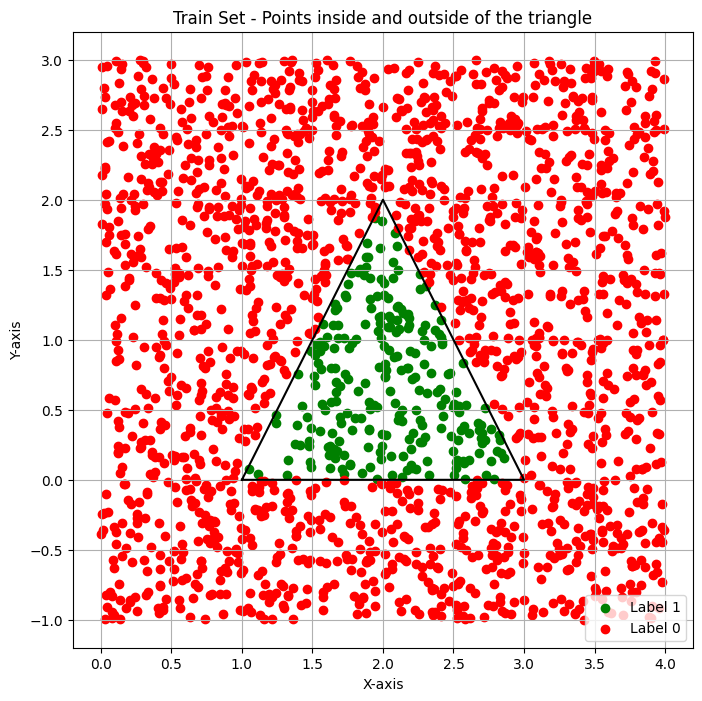
\includegraphics[width=0.4\linewidth]{img/Q1_train_set.png}
		}
	\subfigure[]{
		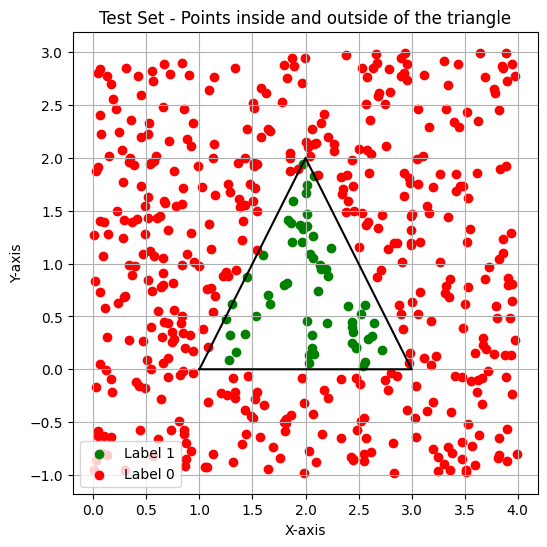
\includegraphics[width=0.4\linewidth]{img/Q1_test_set.png}
		}
	\caption{مجموعه داده تولید شده}
	\label{fig: Q1 data}
\end{figure}

در ادامه یک مدل ‎\lr{MLP}‎‎ روی این مجموعه داده آموزش دیده است و نتایج آن به همراه 
\lr{Decision boundary}‎ 
آن نمایش داده شده است. مدل اول \lr{MLP}‎ با استفاده از توابع \lr{ReLU}‎ ایجاد شده است که جزییات آن به شرح زیر است:
	
\begin{LTR}
\begin{verbatim}
	MLP(
	(layers): Sequential(
	(0): Linear(in_features=2, out_features=8, bias=True)
	(1): ReLU()
	(2): Linear(in_features=8, out_features=64, bias=True)
	(3): ReLU()
	(4): Linear(in_features=64, out_features=8, bias=True)
	(5): ReLU()
	(6): Linear(in_features=8, out_features=1, bias=True)
	(7): Sigmoid()
	)
	)
\end{verbatim}
\end{LTR}
در ادامه مدل فوق با 
\lr{config}
زیر به میزان 150 
\lr{Epoch}
آموزش داده شده است.
\begin{LTR}
	\begin{lstlisting}[language=Python, caption= Configuration]
		device = "cuda" if torch.cuda.is_available else "cpu"
		model = MLP(input_size=2, hidden_size1=8, hidden_size2=64, hidden_size3=8, output_size=1).to(device)
		optimizer = optim.Adam(model.parameters(), lr=0.001)		
		criterion = nn.BCELoss()  # For binary classification
		# DataLoader
		train_loader = DataLoader(TensorDataset(x_train_tensor, y_train_tensor), batch_size=128, shuffle=True)
		test_loader = DataLoader(TensorDataset(x_test_tensor, y_test_tensor), batch_size=512, shuffle=False)
				
	
	\end{lstlisting}
\end{LTR}
کد زیر به منظور اجرای حلقه آموزش نوشته شده است.
در این کد، چندین متغیر برای نگه‌داری اطلاعات مانند تاریخچه‌ی خطاها و معیارهای متریکی مورد استفاده قرار گرفته است. سپس یک حلقه تکرار برای ایپاک‌های مختلف اجرا می‌شود. در هر ایپاک، داده‌های آموزشی بارگذاری شده و مدل در حالت آموزش قرار می‌گیرد. سپس خطا محاسبه می‌شود و بهینه‌سازی می‌شود. معیارهای متریکی مورد نظر نیز برای داده‌های آموزشی توسط توابعی که مستقلا پیاده‌سازی شده‌اند محاسبه می‌شوند. سپس مدل به حالت ارزیابی در آورده می‌شود و برای داده‌های تست خطا و معیارهای متریکی محاسبه می‌شود. در انتهای آموزش، این اطلاعات برای تحلیل و نمایش خروجی‌های آموزش به دست می‌آید. 

\begin{LTR}
	\begin{lstlisting}[language=Python, caption=حلقه آموزش]
num_epochs = 150
train_loss_hist = []
test_loss_hist = []
train_metrics = []
test_metrics = []

for epoch in range(num_epochs):
    loop = tqdm(train_loader)
    model.train()
    train_loss = 0.0
    train_TP, train_FP, train_TN, train_FN = 0, 0, 0, 0

    print("train")
    for inputs, labels in loop:
        inputs = inputs.to(device)
        labels = labels.to(device)
        
        outputs = model(inputs)
        loss = criterion(outputs, labels)

        optimizer.zero_grad()
        loss.backward()
        optimizer.step()
        train_loss += loss.item()

        TP, FP, TN, FN = calculate_metrics(outputs, labels)
        train_TP += TP
        train_FP += FP
        train_TN += TN
        train_FN += FN
        
        loop.set_postfix(
            epoch=epoch+1,
            total_loss=train_loss / len(train_loader),
        )
    
    train_metrics.append((train_TP, train_FP, train_TN, train_FN))
    train_loss_hist.append(train_loss / len(train_loader))
    
    model.eval()
    torch.cuda.empty_cache()
    test_loss = 0.0
    test_TP, test_FP, test_TN, test_FN = 0, 0, 0, 0
    print("Test:")
    
    with torch.no_grad():
        loop = tqdm(test_loader)
        for inputs, labels in loop:
            inputs = inputs.to(device)
            labels = labels.to(device)

            outputs = model(inputs)
            loss = criterion(outputs, labels)
            
            test_loss += loss.item()
            
            TP, FP, TN, FN = calculate_metrics(outputs, labels)
            test_TP += TP
            test_FP += FP
            test_TN += TN
            test_FN += FN
            
            loop.set_postfix(
                loss=loss.item(),
                total_loss=test_loss / len(test_loader),
            )
    test_metrics.append((test_TP, test_FP, test_TN, test_FN))
    test_loss_hist.append(test_loss / len(test_loader))
	\end{lstlisting}
\end{LTR}

\newpage
\subsubsection{نتایج MLP با تابع فعال‌ساز ReLU}

در ‎‎\autoref{fig:Q1 relu training graph}‎ نتایج مربوط به این آموزش نشان داده شده است. همانطور که مشخص است فرآیند آموزش برای مدل ‎\lr{MLP} به درستی انجام شده و مدل روی دیتاست آموزش \lr{over fit}‎ نشده است این درحالی است که میزان متریک‌ها برای هر دو دیتاست به 1 بسیار نزدیک شده است.

\begin{figure}[H]
    \centering
    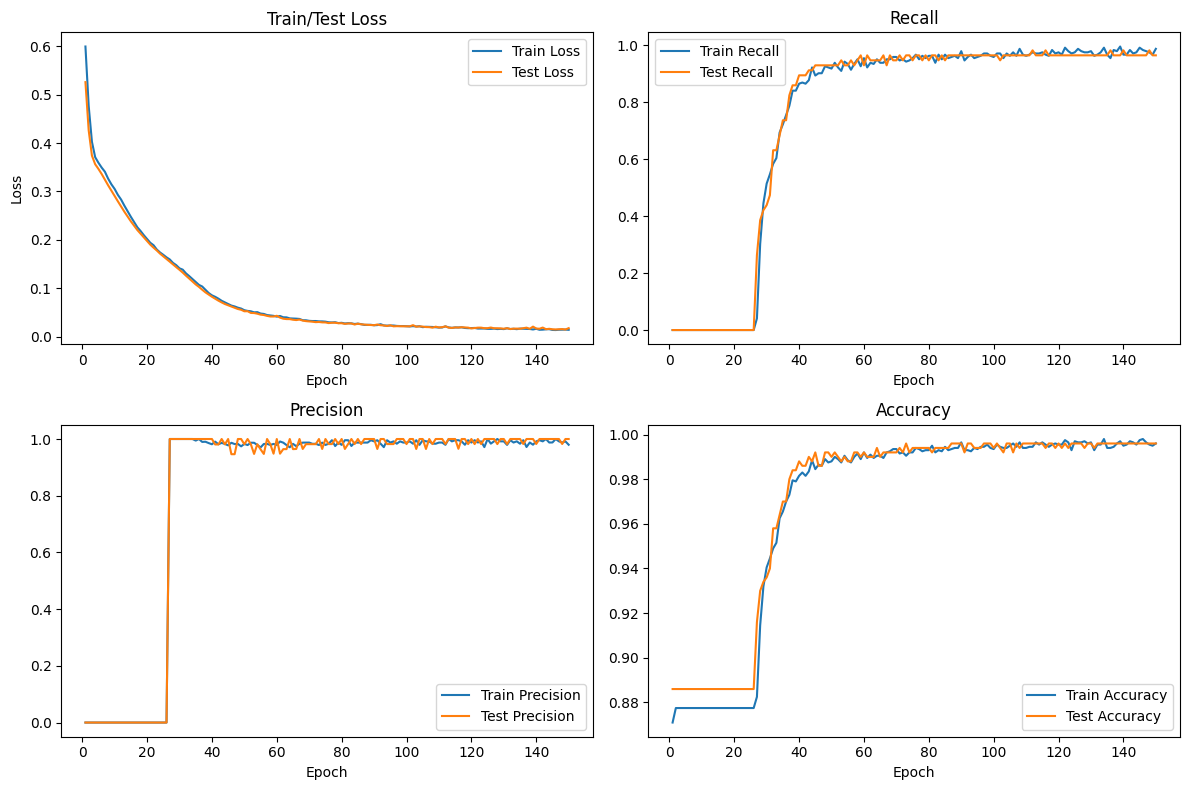
\includegraphics[width=0.7\linewidth]{img/Q1_Relu_metrics_graph.png}
    \caption{نمودارهای متریک و تابع هزینه حین آموزش}
    \label{fig:Q1 relu training graph}
\end{figure}

در ‎\autoref{fig:Q1 relu result}‎ نتیجه عملکرد مدل روی دیتای ارزیابی قابل ملاحضه است و همانطور که مشخص است تنها 2 نقطه در راس بالایی مثلث اشتباه طبقه بندی شده‌اند این درحالی است که هیچ کلاسی که متعلق به داخل دایره بوده، به اشتباه به عنوان یک کلاس در خارج از دایره تشخیص داده نشده است، به عبارت دیگر
\lr{False Negative}
 برابر صفر است و  \lr{‎Precision} برابر 1 است.
 
 در انتها در ‎\autoref{fig:Q1 relu db}‎  مرز تصمیم مدل مشخص است که با توجه با این نمودار مرز حوالی راس پایین سمت راست مثلث از دقت کافی برخوردار نیست.

\begin{figure}[H] 
	\centering
	\subfigure[]{
		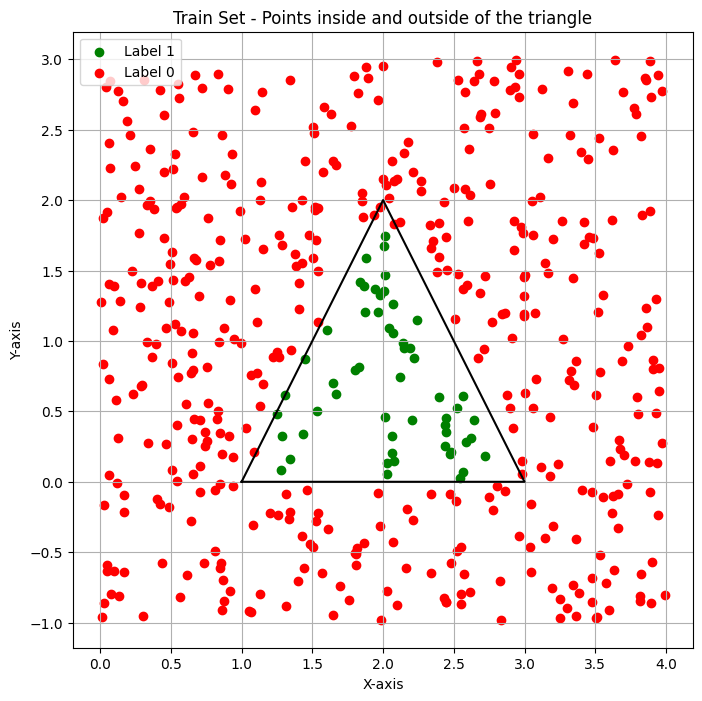
\includegraphics[width=0.4\linewidth]{img/Q1_relu_results.png}
		\label{fig:Q1 relu result}
		}
	\subfigure[]{
		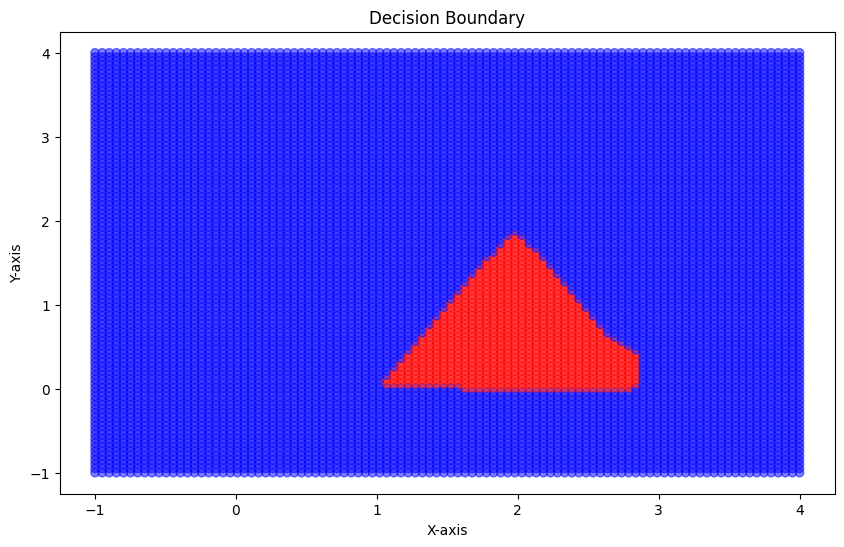
\includegraphics[width=0.4\linewidth]{img/Q1_relu_db.png}
	    \label{fig:Q1 relu db}
		}
\caption{نتایح مدل MLP و مرز تصمیم مربوط به مدل}
\end{figure}


در ‎ \autoref{fig: Q1 relu cm}‎ماتریس درهم‌ریختگی به صورت نرمال و غیرنرمال نشان داده شده است که نشان می‌دهد مدل تنها دو نقطه را که مطعلق به داخل مثل بوده است به اشتباه به عنوان کلاس خارج از مثلث تشخیص داده است.
\begin{figure}[H] 
	\centering
	\subfigure[]{
		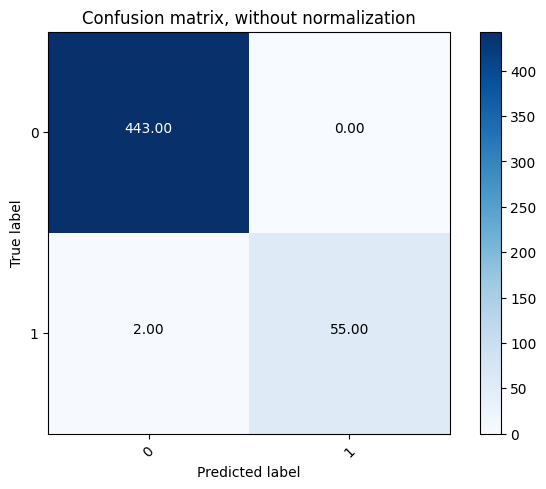
\includegraphics[width=0.4\linewidth]{img/Q1_relu_cm.png}
		}
	\subfigure[]{
		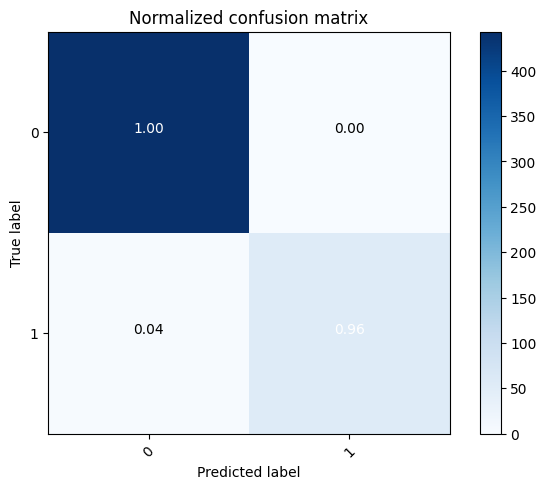
\includegraphics[width=0.4\linewidth]{img/Q1_relu_cmn.png}
		}
	\caption{Confusion Matrix}
	\label{fig: Q1 relu cm}
\end{figure}




\subsubsection{نتایج MLP با تابع فعال‌ساز ELU}

این مدل با استفاده از تابع ELU ساخته شده است و جزییات آن به شرج زیر می‌باشد:

\begin{LTR}
\begin{verbatim}
	MLP(
	  (layers): Sequential(
	    (0): Linear(in_features=2, out_features=8, bias=True)
	    (1): ELU(alpha=1.0)
	    (2): Linear(in_features=8, out_features=64, bias=True)
	    (3): ELU(alpha=1.0)
	    (4): Linear(in_features=64, out_features=8, bias=True)
	    (5): ELU(alpha=1.0)
	    (6): Linear(in_features=8, out_features=1, bias=True)
	    (7): Sigmoid()
	  )
	)
\end{verbatim}
\end{LTR}

در ‎‎\autoref{fig:Q1 elu training graph}‎ نتایج مربوط به این آموزش نشان داده شده است. همانطور که مشخص است فرآیند آموزش برای مدل ‎\lr{MLP} با تابع فعال‌ساز \lr{ELU}‎به درستی انجام شده و مدل روی دیتاست آموزش \lr{over fit}‎ نشده است این درحالی است که شیب نمودار هزینه همچنان کاهشی می‌باشد.در ادامه میزان متریک‌ها برای هر دو دیتاست به 1 بسیار نزدیک شده است.

\begin{figure}[H]
    \centering
    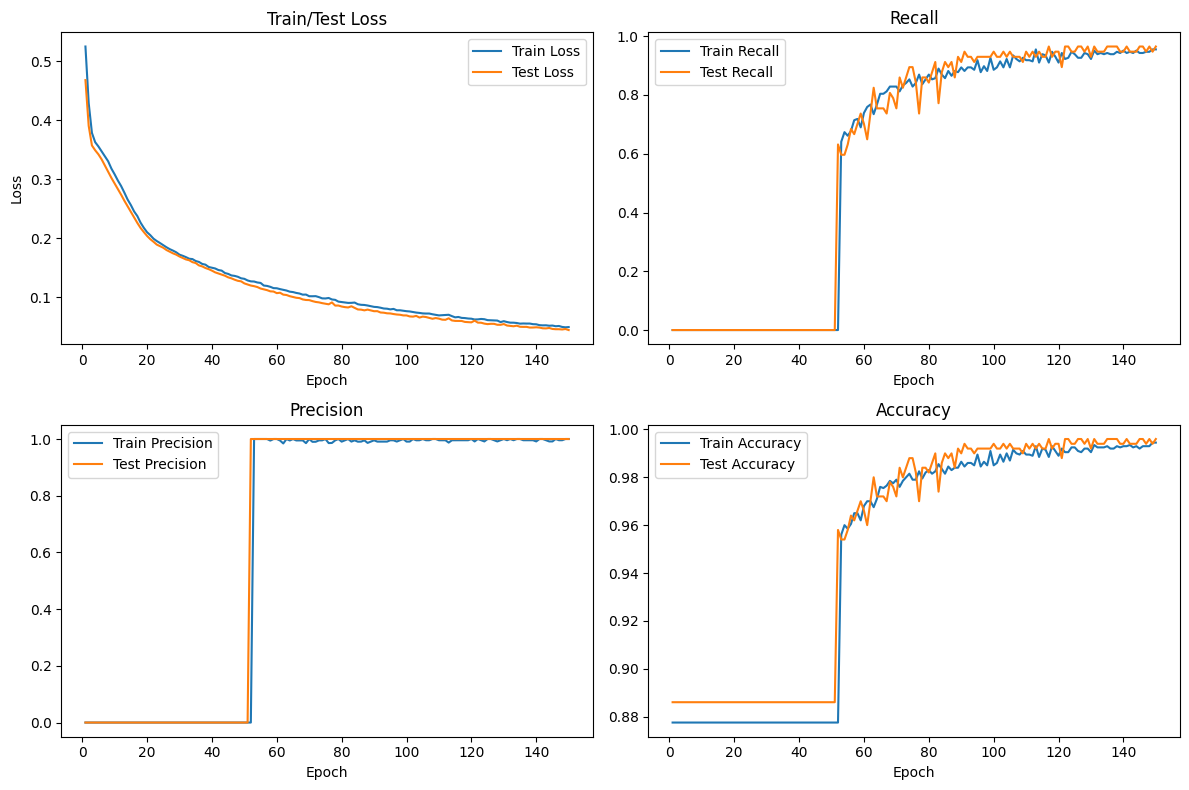
\includegraphics[width=0.7\linewidth]{img/Q1_elu_metrics_graph.png}
    \caption{نمودارهای متریک و تابع هزینه حین آموزش}
    \label{fig:Q1 elu training graph}
\end{figure}

در ‎\autoref{fig:Q1 elu result}‎ نتیجه عملکرد مدل روی دیتای ارزیابی قابل ملاحضه است و همانطور که مشخص است تنها 2 نقطه در راس بالایی مثلث اشتباه طبقه بندی شده‌اند این درحالی است که هیچ کلاسی که متعلق به داخل دایره بوده، به اشتباه به عنوان یک کلاس در خارج از دایره تشخیص داده نشده است، به عبارت دیگر
\lr{False Negative}
 برابر صفر است و  \lr{‎Precision} برابر 1 است.
 
در ‎\autoref{fig:Q1 elu db}‎  مرز تصمیم مدل مشخص است که با توجه به این نمودار و مقایسه آن با ‎\autoref{fig:Q1  relu db}‎، مشخص است که نتایج بدست آمده از این مدل توانایی تعمیم‌پذیری بیشتری دارند و هر سه راس این مثلث به یک شکل هستند.

\begin{figure}[H] 
	\centering
	\subfigure[]{
		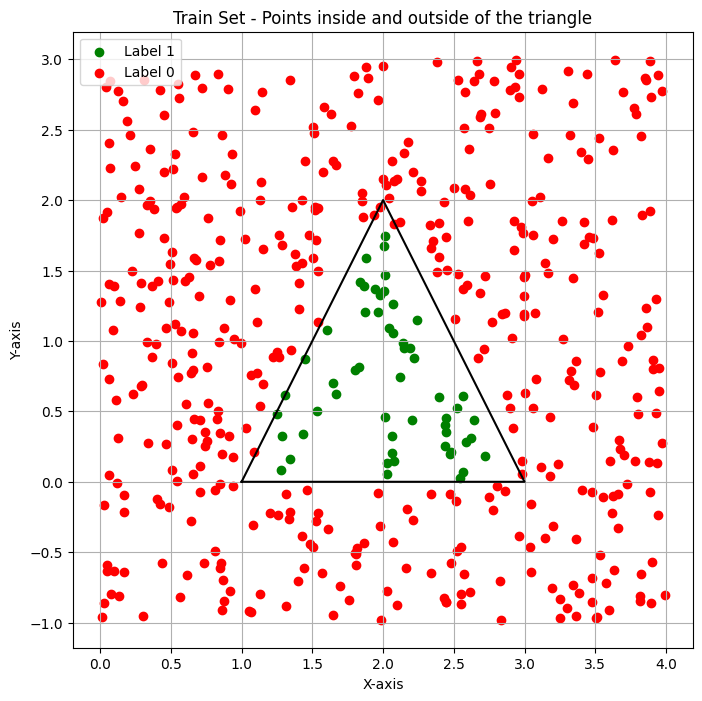
\includegraphics[width=0.4\linewidth]{img/Q1_elu_results.png}
		\label{fig:Q1 elu result}
		}
	\subfigure[]{
		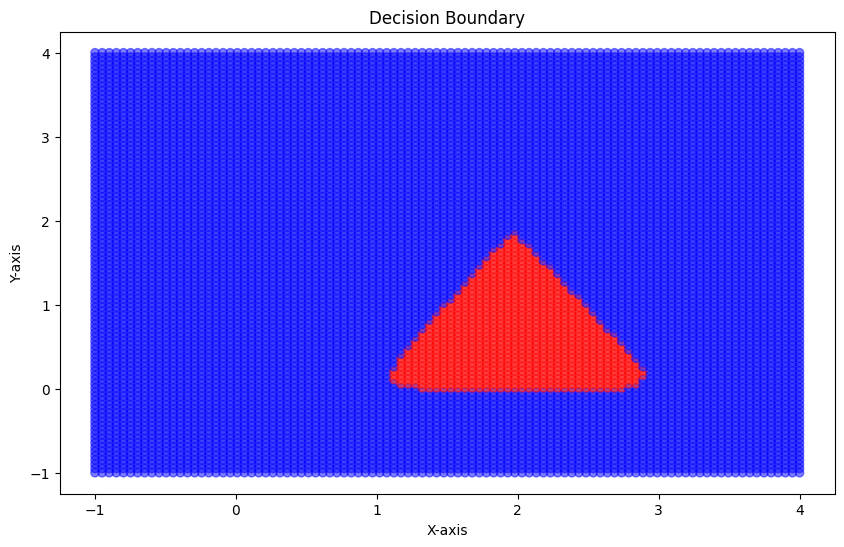
\includegraphics[width=0.4\linewidth]{img/Q1_elu_db.png}
	    \label{fig:Q1 elu db}
		}
\caption{نتایح مدل MLP و مرز تصمیم مربوط به مدل}
\end{figure}


در ‎ \autoref{fig: Q1 elu cm}‎ماتریس درهم‌ریختگی به صورت نرمال و غیرنرمال نشان داده شده است که نشان می‌دهد مدل تنها دو نقطه را که مطعلق به داخل مثل بوده است به اشتباه به عنوان کلاس خارج از مثلث تشخیص داده است.
\begin{figure}[H] 
	\centering
	\subfigure[]{
		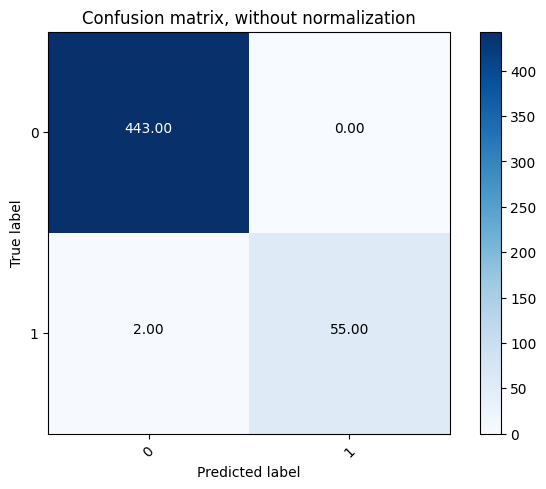
\includegraphics[width=0.4\linewidth]{img/Q1_elu_cm.png}
		}
	\subfigure[]{
		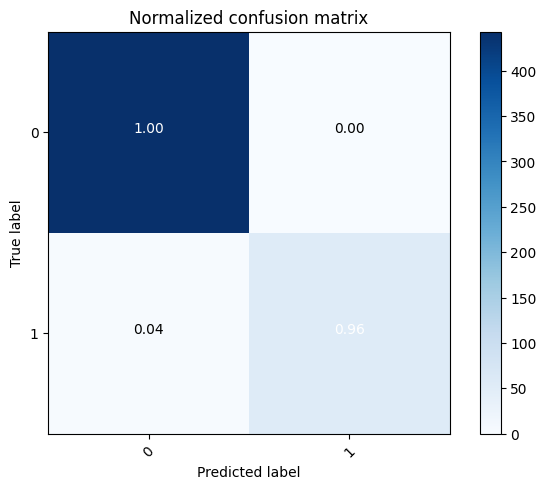
\includegraphics[width=0.4\linewidth]{img/Q1_elu_cmn.png}
		}
	\caption{Confusion Matrix}
	\label{fig: Q1 elu cm}
\end{figure}





\subsubsection{نتایج مدل بر مبنای mcculloch-pitts نرون}

مدل‌های مبتنی بر نرون‌های mcculloch-pitts به ما این امکان را می‌دهند که با استفاده از دانش انسانی، بهترین پاسخ را برای مسئله خود بدست بیاوریم. راه حلی که می‌توانیم نقاط داخل مثلث را شناسایی کنیم حاصل ترکیب AND 3 گزاره متفاوت است؛ هر یک از این گذاره‌ها نشان‌دهنده این است که نقطه مد نظر ما نسبت به خط گذرنده از هر ضلع مثلث چه وضعیتی دارد. بدین منظور باید سه معادله خط بدست آوریم و با قرار دادن نقاط اطراف خط مشخص کنیم که تغییر علامت چه زمانی رخ می‌دهد و با چه ترکیب منطقی از این تغییر علامت‌ها می‌توانیم مثلث را پیدا کنیم.
 

در ‎‎\autoref{fig:Q1 elu training graph}‎ نتایج مربوط به این آموزش نشان داده شده است. همانطور که مشخص است فرآیند آموزش برای مدل ‎\lr{MLP} با تابع فعال‌ساز \lr{ELU}‎به درستی انجام شده و مدل روی دیتاست آموزش \lr{over fit}‎ نشده است این درحالی است که شیب نمودار هزینه همچنان کاهشی می‌باشد.در ادامه میزان متریک‌ها برای هر دو دیتاست به 1 بسیار نزدیک شده است.
روش محاسبه هر یک از این معادلات خط با قرار دادن یک جفت از راس‌های مثلث در معادله زیر می‌باشد:

\begin{align}
y &= w(x-x_1)+y_1 ,\quad w = \frac{y_1-y_2}{x_1-x_2}
\end{align}
با استفاده از رابطه فوق سه جفت مقدار برای هر معادله خط بدست آمد که این مقادیر عبارتند از
$(-2,1)$، $(2,1)$ و $(0,1)$
که سه ضلع مثلث را تشکیل می‌دهند. در ادامه یک نرون لازم است تا عملیات منطقی AND را انجام دهد. با جایگذاری نقاط مختلف از صفحه در معادلات خط بدست آمده و مقایسه آنها رابطه منطقی زیر بدست می‌آید:
$$l_1'+l_2'+l_3$$

مدل مرتبط با روابط فوق به شکل زیر در پایتون قابل پیاده‌سازی می‌باشد:
 \begin{LTR}
 	\begin{lstlisting}[language=Python, caption=حلقه آموزش]
		#define muculloch pitts
		class McCulloch_Pitts_neuron():
		
		  def __init__(self , weights ,bias, threshold):
		    self.weights = np.array(weights).reshape(-1, 1)     #define weights
		    self.threshold = threshold    #define threshold
		    self.bias = np.array(bias)
		    
		  def model(self , x):
		    #define model with threshold
		    return (x.T @ self.weights + self.bias >= self.threshold).astype(int)
		    
		def model(x):
		    neur1 = McCulloch_Pitts_neuron([-2, 1],2, 0)
		    neur2 = McCulloch_Pitts_neuron([2, 1], -6, 0)
		    neur3 = McCulloch_Pitts_neuron([0, 1], 0, 0)
		    neur4 = McCulloch_Pitts_neuron([1, 1, 1], 0, 3)
		
		    z1 = neur1.model(np.array(x))
		    z2 = neur2.model(np.array(x))
		    z3 = neur3.model(np.array(x))
		    z4 = np.squeeze(np.array([1-z1, 1-z2, z3]), axis=-1)
		    z4 = neur4.model(z4)
		
		    # 3 bit output
		    # return str(z1) + str(z2)
		    return z4
		
 	\end{lstlisting}
 \end{LTR}


همانطور که در ‎\autoref{fig:Q1 mp db}‎ مشخص است یک مثلث دقیق بدست آمده است و انتظار می‌رود که نتایج ماتریس درهم‌ریختگی آن بهترین وضعیت ممکن باشد که این مسئله در ‎\autoref{fig: Q1 mp cm}‎ قابل مشاهده است.

\begin{figure}[H] 
	\centering
		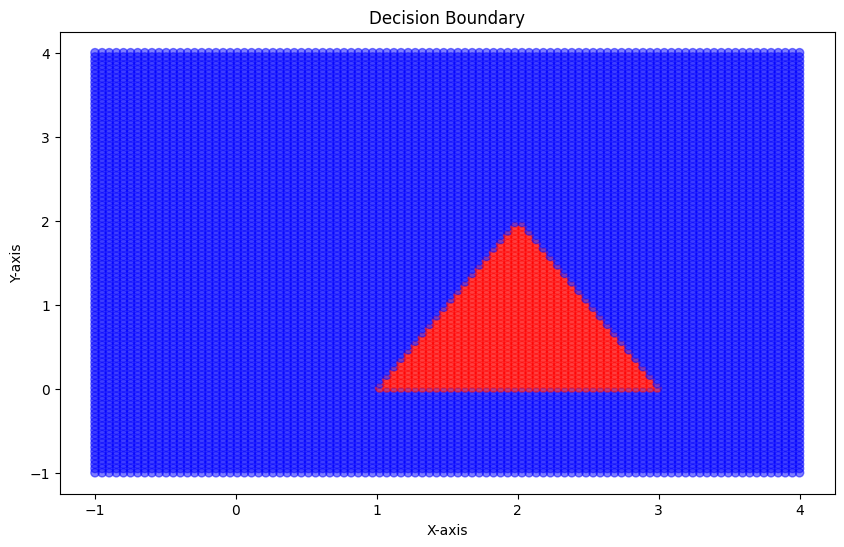
\includegraphics[width=0.4\linewidth]{img/Q1_cp_db.png}
		\label{fig:Q1 mp db}
\caption{mcculloch-pitts و مرز تصمیم مربوط به مدل}
\end{figure}


\begin{figure}[H] 
	\centering
	\subfigure[]{
		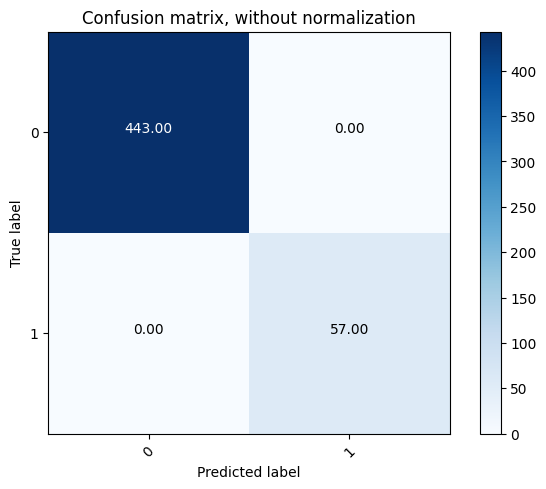
\includegraphics[width=0.4\linewidth]{img/Q1_cp_cm.png}
		}
	\subfigure[]{
		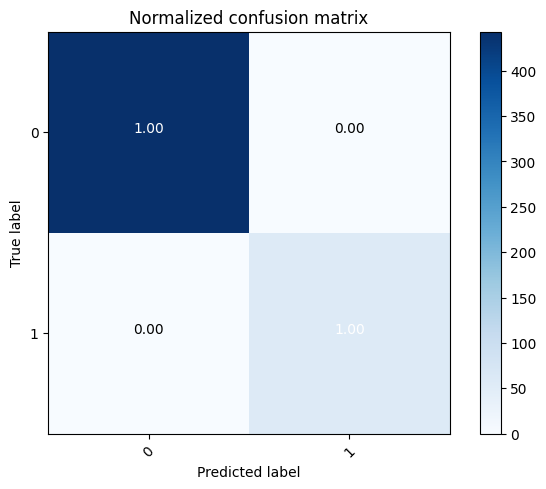
\includegraphics[width=0.4\linewidth]{img/Q1_cp_cmn.png}
		}
	\caption{Confusion Matrix}
	\label{fig: Q1 mp cm}
\end{figure}

%%%%%%%%%%%%%%%%%%%%%%%%%%%%%%%%%%%%%%%%%%%%%%%%%%%%%% Q2

\section{سوال2}

\subsection{بخش اول}

{\large \textbf{سوال}:} 

در مورد دیتاست CWRU Bearin و عیوب موجود توضیح دهید. 

{\large \textbf{پاسخ}:} 

دیتاست استفاده شده برای این پروژه، دیتاست CWRU Bearing است. این دیتاست شامل داده‌های ارتعاشی از بلبرینگ‌ها در شرایط مختلف، شامل حالت‌های سالم و معیوب است. در این مینی‌پروژه، ما بر روی داده‌های بخش
 \lr{12k Drive End Bearing Fault Data} 
 تمرکز می‌کنیم.
علاوه بر داده‌های استفاده شده در مینی‌پروژه قبلی، ما اکنون دو کلاس جدید
 \lr{OR007@6\_1} و \lr{B007\_1}
 از بلبرینگ‌های معیوب را اضافه می‌کنیم. این گسترش پیچیدگی و تنوع بیشتری به داده‌ها اضافه می‌کند و امکان تحلیل جامع‌تر و آموزش مدل قوی‌تر را فراهم می‌کند.
انواع داده‌های معیوب و توضیحات آن به شرح زیر می‌باشد:
\begin{itemize}
    \item \textbf{سالم:} داده‌هایی که نشان‌دهنده بلبرینگ‌های در عادی خوب هستند.
    \item \textbf{کلاس معیوب 1 \lr{OR007@6\_1}:} این عیوب در قسمت بیرونی بلبرینگ رخ می‌دهد و می‌تواند ارتعاش و نویز قابل توجهی ایجاد کند که عملکرد کلی ماشین‌آلات را تحت تاثیر قرار می‌دهد.
    \item \textbf{کلاس معیوب 2 \lr{B007\_1}:} این عیوب در سطح بلبرینگ‌ها رخ می‌دهد و با نامنظمی‌هایی در سطح بلبرینگ‌ها همراه است.
    \item \textbf{کلاس معیوب 3 \lr{(IR007\_1)}:} این عیوب در قسمت داخلی بلبرینگ رخ می‌دهد و باعث ایجاد ناهنجاری در عملکرد کلی بلبرینگ می‌شود.
\end{itemize}

\subsection{پیش‌پردازش}

کد زیر یک چنجره به طول 
\texttt{len\_data}
را روی سری زمانی عبور می‌دهد و داده7ها را به شکل یک ماتریس 
$(n, \texttt{len\_data})$
ایجاد می‌کند که مقدار n با توجه به تعداد داده موجود در فایل دیتا بستگی دارد. سپس با توجه به متغییر ‎\texttt{n‎\_samples} تعداد نمونه دلخواه را جدا می‌کنیم. به دلیل اینکه در این مسئله تصمیم به آموزش یک شبکه عصبی داریم بیشترین تعداد داده ممکن را از دیتاست استخراج می‌کنیم که برابر 600 نمونه پنجره با طول 200 است.‎
\begin{LTR}
	\begin{lstlisting}[language=Python, caption=Sliding Window]
	n_samples = 600
	len_data = 200
	
	normal_data_matrix = normal_data[:-(normal_data.shape[0] % len_data)].reshape(-1, len_data)
	fault1_data_matrix = fault1_data[:-(fault1_data.shape[0] % len_data)].reshape(-1, len_data)
	fault2_data_matrix = fault2_data[:-(fault2_data.shape[0] % len_data)].reshape(-1, len_data)
	fault3_data_matrix = fault3_data[:-(fault3_data.shape[0] % len_data)].reshape(-1, len_data)
	\end{lstlisting}
\end{LTR}

در ادامه خروجی کد فوق نشان داده شده است.
\begin{LTR}
\begin{verbatim}
(2419, 200)
(609, 200)
(607, 200)
(612, 200)
\end{verbatim}
\end{LTR}

در ادامه با استفاده از کد زیر 
\lr{feature}های
ممکن را از هر پنجره از داده استخراج می‌کنیم و سپس ویژگی‌هایی که مد نظر هست را انتخاب می‌کنیم.

\begin{LTR}
	\begin{lstlisting}[language=Python, caption=Feature Extraction and Feature Selection]
def feature_extraction(data):
    features = {}
    # Standard Deviation
    features['Standard Deviation'] = np.std(data, axis=1)
    # Peak
    features['Peak'] = np.max(np.abs(data), axis=1)
    # Skewness
    features['Skewness'] = scipy.stats.skew(data, axis=1)
    # Kurtosis
    features['Kurtosis'] = scipy.stats.kurtosis(data, axis=1)
    # Crest Factor (peak divided by RMS)
    rms = np.sqrt(np.mean(np.square(data), axis=1))
    features['Crest Factor'] = features['Peak'] / rms
    # Clearance Factor (peak divided by the mean of the square root of the absolute values)
    features['Clearance Factor'] = features['Peak'] / np.mean(np.sqrt(np.abs(data)), axis=1)
    # Peak to Peak
    features['Peak to Peak'] = np.ptp(data, axis=1)
    # Shape Factor (RMS divided by the mean of the absolute values)
    features['Shape Factor'] = rms / np.mean(np.abs(data), axis=1)
    # Impact Factor (peak divided by mean)
    features['Impact Factor'] = features['Peak'] / np.mean(data, axis=1)
    # Square Mean Root (the square root of the mean of the squares)
    features['Square Mean Root'] = rms
    # Mean
    features['Mean'] = np.mean(data, axis=1)
    # Absolute Mean
    features['Absolute Mean'] = np.mean(np.abs(data), axis=1)
    # Root Mean Square
    features['Root Mean Square'] = rms
    # Impulse Factor (peak divided by the absolute mean)
    features['Impulse Factor'] = features['Peak'] / features['Absolute Mean']
    return features
normal_features = pd.DataFrame(feature_extraction(normal_data_matrix))
fault1_features = pd.DataFrame(feature_extraction(fault1_data_matrix))
fault2_features = pd.DataFrame(feature_extraction(fault2_data_matrix))
fault3_features = pd.DataFrame(feature_extraction(fault3_data_matrix))
normal_features['Label'] = 0
fault1_features['Label'] = 1
fault2_features['Label'] = 2
fault3_features['Label'] = 3

selected_features = ['Standard Deviation', 'Peak', 'Skewness', 'Kurtosis',
                     'Crest Factor', 'Mean', 'Root Mean Square',
                     'Impulse Factor','Square Mean Root','Shape Factor','Label']

main_df = pd.concat([normal_features, fault1_features, fault2_features, fault3_features], ignore_index=True)
df = main_df[selected_features]
	\end{lstlisting}
\end{LTR}

در ادامه تقسیم دیتاست به 3 زیرمجموعه آموزش، ارزیابی و آزمون انجام شده است که به موجب آن ابتدا به صورت تصادفی 
\lr{shuffle}
می‌شوند و پس از آن یک بار به صورت عادی و بار بعدی به صورت 
\texttt{stratify}
تقسیم داده انجام می‌شود. با مشخص کردن آرگمان 
\texttt{stratify}
باعث می‌شویم که توزیع داده در زیرمجموعه آزمون و ارزیابی بهم نریزد. تقسیم مجموعه داده با استفاده از آرگمان فوق باعث بهبود نتایج آموزش مدل نسبت به شرایطی که انتخاب هر زیرمجموعه به صورت کاملا تصادفی بوده، شده است.

اضافه کردن مجموعه داده اعتبارسنجی و بررسی تابع هزینه روی این مجموعه داده حین آموزش، موجب آن میشود که از اتفاق افتادن 
\lr{over-fitting}
جلوگیری شود.
\begin{LTR}
	\begin{lstlisting}[language=Python, caption=Train\, Validatiaon\, Test Split]
df_shuffled = df.sample(frac=1).reset_index(drop=True)

X = df_shuffled.drop('Label', axis=1)
y = df_shuffled['Label']

# X_train_raw, X_test_raw, y_train, y_test = train_test_split(X, y, test_size=0.20, random_state=53)
# X_train_raw, X_val_raw, y_train, y_val = train_test_split(X_train_raw, y_train, test_size=0.25, random_state=53)
X_train_raw, X_test_raw, y_train, y_test = train_test_split(X, y, test_size=0.20, stratify=y, random_state=53)
X_train_raw, X_val_raw, y_train, y_val = train_test_split(X_train_raw, y_train, test_size=0.25, stratify=y_train, random_state=53)
	\end{lstlisting}
\end{LTR}

\subsection{بخش دوم}
\label{section2}
 در ادامه مجموعه داده بدست آمده را نرمال می‌کنیم، باید توجه داشت که مقادیر میانگین و واریانسی که به منظور نرمال کردن مجموعه داده ارزیابی و آزمون در نظر گرفته شده است از مجموعه داده آموزش بدست آمده است. در انتها متناسب با عدد موجود در Label هر داده، یک آرایه به صورت 
One-hot
به آن داده اختصاص داده شده است.
 
\begin{LTR}
	\begin{lstlisting}[language=Python, caption=Normalization and One-hot]
 X_train, X_train_max, X_train_min = min_max_normalization(X_train_raw)
 X_test, _, _ = min_max_normalization(X_test_raw,X_train_max,X_train_min)
 X_val, _, _ = min_max_normalization(X_val_raw,X_train_max,X_train_min)
 
 X_train = torch.tensor(X_train.to_numpy(), dtype=torch.float32)
 X_val = torch.tensor(X_val.to_numpy(), dtype=torch.float32)
 X_test = torch.tensor(X_test.to_numpy(), dtype=torch.float32)
 
 y_train = torch.tensor(y_train.to_numpy(), dtype=torch.long)
 y_val = torch.tensor(y_val.to_numpy(), dtype=torch.long)
 y_test = torch.tensor(y_test.to_numpy(), dtype=torch.long)
 
 # Perform one-hot encoding
 y_train = torch.nn.functional.one_hot(y_train, num_classes=4).float()
 y_val = torch.nn.functional.one_hot(y_val, num_classes=4).float()
 y_test = torch.nn.functional.one_hot(y_test, num_classes=4).float()
	\end{lstlisting}
\end{LTR} 

در ادامه یک مدل MLP با سه لایه پنهان ایجاد می‌کنیم که شرح تعداد نرون‌های آن در کد زیر آمده است سپس با مقدار‌دهی اولیه مدل، یک شی در محیط برنامه نویسی ایجاد می‌کنیم. پارامتر بعدی که در آموزش این مدل استفاده شده است تابع هزینه 
\texttt{CrossEntropyLoss}
است که یک شی از آن با مقادیر پیش‌فرض ایجاد شده است. تابع بهینه ساز این مدل از الگوریتم Adam پیروی میکند که با گام اموزشی اولیه 
$0.001 $
شروع به بهینه کردن مدل می‌کند و در ادامه با استفاده از تابع 
\texttt{lr\_scheduler}
اگر طی 15 
Epoch
 بهبودی در نتایج تابع هزینه روی مجموعه داده ارزیابی رخ ندهد، میزان گام آموزشی 0.1 مقدار قبلی خود خواهد شد. 
\begin{LTR}
	\begin{lstlisting}[language=Python, caption=Model and Configuration]
class MLP(nn.Module):
    def __init__(self, input_dim, output_dim):
        super(MLP, self).__init__()
        self.hidden1 = nn.Linear(input_dim, 32)
        self.hidden2 = nn.Linear(32, 64)
        self.output = nn.Linear(64, output_dim)
        self.relu = nn.ReLU()
        self.softmax = nn.Softmax(dim=1)

    def forward(self, x):
        x = self.relu(self.hidden1(x))
        x = self.relu(self.hidden2(x))
        x = self.output(x)
        x = self.softmax(x)
        return x
        
# Initialize the model, loss function, and optimizer
model = MLP(input_dim=X_train.shape[1], output_dim=len(set(y)))
criterion = nn.CrossEntropyLoss()
optimizer = optim.Adam(model.parameters(), lr=0.001)
scheduler = optim.lr_scheduler.ReduceLROnPlateau(optimizer, mode='min', factor=0.1, patience=15, verbose=True)
	\end{lstlisting}
\end{LTR}         
        
در انتها مدل با استفاده از کد زیر آموزش داده می‌شود؛ باید توجه داشته که کد زیر با بررسی تغییرات تابع هزینه دستاست ارزیابی، میزان بهبود آن را بررسی می‌کند و اگر به ازای 30 
Epoch
بهبود محسوس رخ ندهد فرایند آموزش متوقف می‌شود.
\begin{LTR}
	\begin{lstlisting}[language=Python, caption=Train Loop]       
# Training loop with early stopping
num_epochs = 500
patience = 30
best_val_loss = float('inf')
epochs_without_improvement = 0
Best_model = None

# Metrics storage
train_losses = []
val_losses = []
train_accuracies = []
val_accuracies = []

for epoch in range(num_epochs):
    model.train()
    train_loss = 0.0
    train_correct = 0
    total_train = 0

    for inputs, labels in train_loader:
        optimizer.zero_grad()
        outputs = model(inputs)
        loss = criterion(outputs, labels)
        loss.backward()
        optimizer.step()
        train_loss += loss.item()

        _, preds = torch.max(outputs, 1)
        _, targets = torch.max(labels,1)
        train_correct += (preds == targets).sum().item()
        total_train += labels.size(0)

    train_loss /= len(train_loader)
    train_accuracy = train_correct / total_train
    train_losses.append(train_loss)
    train_accuracies.append(train_accuracy)

    model.eval()
    val_loss = 0.0
    val_correct = 0
    total_val = 0
    with torch.no_grad():
        for inputs, labels in val_loader:
            outputs = model(inputs)
            loss = criterion(outputs, labels)
            val_loss += loss.item()

            _, preds = torch.max(outputs, 1)
            _, targets = torch.max(labels,1)
            val_correct += (preds == targets).sum().item()
            total_val += labels.size(0)

    val_loss /= len(val_loader)
    val_accuracy = val_correct / total_val
    val_losses.append(val_loss)
    val_accuracies.append(val_accuracy)

    print(f'Epoch {epoch+1}/{num_epochs}, Train Loss: {train_loss:.4f}, Val Loss: {val_loss:.4f}, Train Accuracy: {train_accuracy:.4f}, Val Accuracy: {val_accuracy:.4f}')

    scheduler.step(val_loss)
    
    if  best_val_loss - val_loss > 1e-3:
        best_val_loss = val_loss
        torch.save(model.state_dict(), 'best_model.pth')
        epochs_without_improvement = 0
    else:
        epochs_without_improvement += 1

    if epochs_without_improvement >= patience:
        print(f'Early stopping triggered after {epoch+1} epochs.')
        break
	\end{lstlisting}
\end{LTR}         
        
\subsubsection{نتایج}
پس از آموزش مدل با 
configuration 
که در بالا مطرح شد نتایج بدست آمده از تابع هزینه و متریک 
Accuracy
در 
\autoref{fig:Q2 result basic}
نشان داده شده است. در این آموزش، با گذشتن 258 
Epoch
بهبودی در میزان تابع هزینه دیتاست ارزیابی مشاهده نشده است و فرایند آموزش
early stop 
شده است. همانطور که مشخص است میزان accuracy این مجموعه داده آموزش و ارزیابی در طی فرایند آموزش به حدود یک نزدیک شده است و همانطور که از این نمودار مشخص است، بهینه سازی این مدل در 2 نقطه به 
local extremum 
رسیده است و برای حدود چند 
Epoch
بهبودی در نتایج این متریک مشاهده نمی‌شود. 
\begin{figure}[H]
\centering
\includegraphics[width=1\linewidth]{"img/Q2/result basic"}
\caption{نتایج آموزش مدل MLP}
\label{fig:Q2 result basic}
\end{figure}

به منظور تحلیل بهتر نتایح بدست آمده از آموزش این مدل متریک‌ها و معیارهای دیگری علاوه بر 
Accuracy 
مورد نیاز است زیرا که متریک 
Accuracy 
با در نظر گرفتن کلاس‌های نرمالی که به درستی تشخیص داده شده‌اند در فرمول خود، باعث کاهش اثر نمونه‌هایی که به اشتباه تشخیص داده‌شده‌اند می‌شود بنابراین متریک‌های دیگری مورد نیاز است که در ادامه نتایج مدل را برحسب 
Recall و Precision و F-1 Score
و ماتریس درهم‌ریختگی روی مجموعه داده آزمون بررسی می‌شود.

نتایج آموزش مدل روی داده آزمون در 
\autoref{fig:Q2 cm basic}
و
\autoref{Q2 basic result}
نشان دهنده عملکرد بسیار خوب این مدل می‌باشد که تمام نمونه‌ها را به درستی تشخیص داده است.
 
\begin{LTR}
\label{Q2 basic result}
\begin{verbatim}
              precision    recall  f1-score   support

           0       1.00      1.00      1.00       359
           1       1.00      1.00      1.00       375
           2       1.00      1.00      1.00       348
           3       1.00      1.00      1.00       358

    accuracy                           1.00      1440
   macro avg       1.00      1.00      1.00      1440
weighted avg       1.00      1.00      1.00      1440
\end{verbatim}
\end{LTR}

\begin{figure}[H]
\centering
\includegraphics[width=0.5\linewidth]{"img/Q2/cm basic"}
\caption{Confiusion Matrix}
\label{fig:Q2 cm basic}
\end{figure}

\subsection{بخش سوم}

در ادامه با استفاده از کد زیر 2 مدل جدید با 
configuratinهای 
جدید ایجاد می‌کنیم که در مدل اول تنها تابع هزینه به 
\texttt{L1Loss}
تبدیل شده و در مدل دوم علاوه بر آن بهینه‌ساز به الگوریتم 
\texttt{SGD}
تغییر یافته است.
\begin{LTR}  
	\begin{lstlisting}       
# Model 1
model = MLP(input_dim=X_train.shape[1], output_dim=len(set(y)))
criterion = nn.L1Loss()
optimizer = optim.Adam(model.parameters(), lr=0.1)
scheduler = optim.lr_scheduler.ReduceLROnPlateau(optimizer, mode='min', factor=0.1, patience=15, verbose=True)

# model 2
model = MLP(input_dim=X_train.shape[1], output_dim=len(set(y)))
criterion = nn.L1Loss()
optimizer = optim.SGD(model.parameters(), lr=0.1)
scheduler = optim.lr_scheduler.ReduceLROnPlateau(optimizer, mode='min', factor=0.1, patience=15, verbose=True)
	\end{lstlisting}
\end{LTR}         
        
\subsubsection{نتایج}

 با توجه به نمودارهای موجود در 
\autoref{fig:Q2 metric-of-opt-loss} و \autoref{fig:Q2 loss-of-opt-loss}
مشخص می‌شود که تغییر تابع هزینه به تنهایی می‌تواند به شدت روی عملکرد مدل تاثیر بگذارد؛ این مسئله با بررسی نمودارهای نارنجی که مربوط به مدل با تابع هزینه
\texttt{L1Loss} و 
بهینه ساز
\texttt{Adam}
است مشخص می‌شود. در آموزش این مدل مشخص می‌شود که یک نقطه بهینه محلی پیدا شده است که مدل نتوانسته است از آن خارج شود و مقدار 
Accuracy
برابر 75‎\% شده است که نشان دهنده افت شدید این متریک نسبت به شرایطی است که تابع هزینه از نوع
\texttt{CrossEntropyLoss}
است.

در ادامه با تغییر بهینه‌ساز در فرایند آموزش به 
\texttt{SGD}
نشان داده می‌شود که دوباره مدل به نتیجه مطلوب می‌رسد اما باید این نکته را در نظر داشته که بابت رسیدن به این نتیجه نیاز است که 500 
Epoch
طی شود که خیلی بیشتر از تعداد 
Epoch
طی شده در فرایند آموزش نشان داده‌شده در 
\autoref{section2}
 می‌باشد. نکته حائز اهمیت در نمودارهای ‎
 \autoref{fig:Q2 loss-of-opt-loss}
 این است که آموزشی که با نمودار آبی نشان داده شده است همچنان می‌تواند آموزش داده شود و داری شیب نزولی هم در نمودار آموزش و هم در نمودار ارزیابی است.
\begin{figure}[H]
\centering
\includegraphics[width=1\linewidth]{"img/Q2/loss of opt loss"}
\caption{تابع هزینه آموزش مدل MLP با بهینه ساز و تابع هزینه جدید}
\label{fig:Q2 loss-of-opt-loss}
\end{figure}

\begin{figure}[H]
\centering
\includegraphics[width=1\linewidth]{"img/Q2/metric of opt loss"}
\caption{متریک‌های آموزش مدل MLP با بهینه ساز و تابع هزینه جدید}
\label{fig:Q2 metric-of-opt-loss}
\end{figure}

در ادامه به منظور مقایسه عملکرد مدلی که تابع هزینه و الگوریتم بهینه‌سازی آن عوض شده است با مدل قبلی، ماتریس درهم‌ریختگی را روی مجموعه داده تست محاسبه می‌کنیم که در ‎
\autoref{fig:Q2 cm-of-opt-loss}
نمایش آن قابل ملاحظه است. همانطور که از این ماتریس مشخص است، مدلی که تابع هزینه و بهینه ساز آن تغییر کرده است در 4 نمونه از کلاس سالم را به اشتباه متعلق به کلاس 2 تشخیص داده است و 1 نمونه از کلاس 3 را متعلق به کلاس 1 تشخیص داده است که در مجموع 5 خطا دارد؛ این درحالی است که مدل بدست آمده در
\autoref{section2}
هیچ خطایی روی محموعه داده آزمون نداشته است، بنابراین تغییر تابع هزینه و یا بهینه ساز می‌تواند موجب کاهش عملکرد مدل در این مسئله بشود.  
\begin{figure}[H]
\centering
\includegraphics[width=0.5\linewidth]{"img/Q2/cm of opt loss"}
\caption{ماتریس درهم‌ریختگی روی داده‌های آزمون}
\label{fig:Q2 cm-of-opt-loss}
\end{figure}

























\bibliographystyle{plain}
\bibliography{references}
\end{document}

